\chapter*{Introducción}
\addcontentsline{toc}{chapter}{Introducción}
\chaptermark{Introducción}


La velocidad a la que evoluciona la tecnología es cada vez mayor, por lo que necesitamos seguir desarrollando software
y crear aplicaciones para aprovechar al máximo las herramientas de que disponemos. Una de estas tecnologías es la
Realidad Extendida (XR - \textit{Extended Reality}) con todos sus niveles de interacción y, para cada tarea, necesitamos encontrar la respuesta más adecuada a las necesidades.

En este informe voy a mostrar los resultados del proyecto realizado durante mi período de práctica profesional dentro del instituto Fraunhofer IPK en Berlín, Alemania.
Para ello, voy a exponer los grandes bloques conceptuales que componen este proyecto, el estado del arte actual, el trabajo realizado, ejemplos de código, esquemas de datos y conclusiones personales.

\begin{figure}[ht]
    \begin{center}
       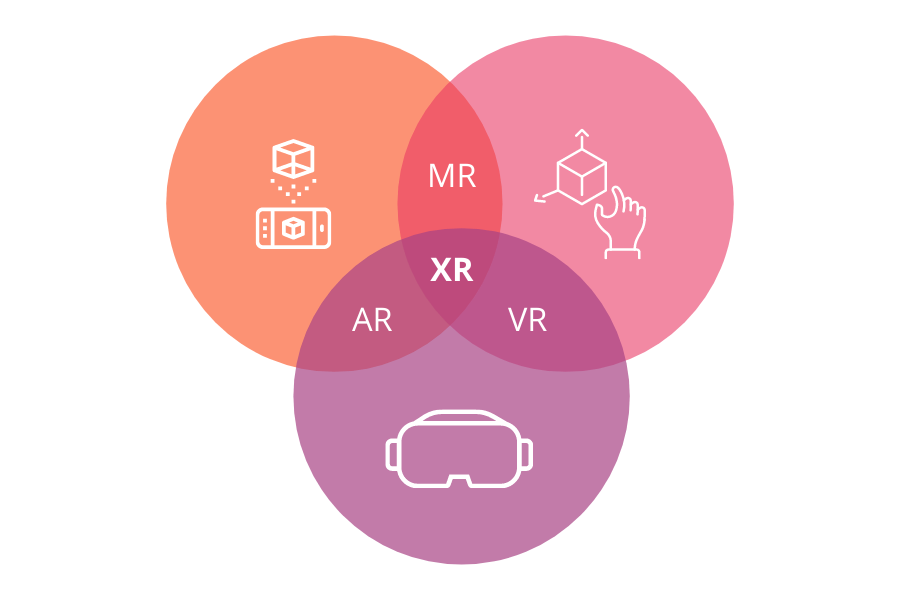
\includegraphics[width=0.6\linewidth]{introduction/figures/Extended-Reality.png}
    \end{center}
    \caption[Realidad Extendida y sus variantes]
    {\footnotesize Realidad Extendida y sus variantes}
    \label{fig:mufigure1}
 \end{figure}


\section{Realidad Extendida}

RX es un término emergente que engloba todas las tecnologías inmersivas. Las que ya existen -realidad aumentada (RA), realidad virtual (RV) y realidad mixta (RM)- y las que están por surgir. Todas las tecnologías inmersivas amplían la realidad que experimentamos mezclando los mundos virtual y ``real'' o creando una experiencia totalmente inmersiva.
\textbf{Reciente investigación sostiene : }

\boitemagique{Cuándo se espera que la RX se generalice?}{
Más del 60\% de los accionistas de empresas de productos RX consideran que se volverá masiva en los próximos 5 años. \cite[]{ExtendedReality}
}

Los diferentes tipos de Realidad Extendida son:
\begin{itemize}
\item \textbf{Realidad Aumentada (\uppercase{RA})}

En la realidad aumentada, la información y los objetos virtuales se superponen al mundo real.
Esta experiencia realza el mundo real con detalles digitales como imágenes, texto y animación.
Se puede acceder a la experiencia a través de pantallas, tablets y smarthpones.
Esto significa que los usuarios no están aislados del mundo real y pueden seguir interactuando y viendo lo que ocurre delante de ellos. Los ejemplos más conocidos de RA son el juego Pokemon GO, que superpone criaturas digitales al mundo real, o los filtros de Snapchat, que colocan en la cabeza objetos digitales como sombreros o gafas.
\item \textbf{Realidad Virtual (\uppercase{RV})}

A diferencia de la realidad aumentada, en una experiencia de realidad virtual
los usuarios se sumergen por completo en un entorno digital simulado.
Las personas deben ponerse un casco de realidad virtual o una pantalla montada en la cabeza para obtener una visión de 360 grados de un mundo artificial que
que engaña a su cerebro haciéndole creer que está, por ejemplo, caminando sobre la luna, nadando bajo el océano o adentrándose en cualquier nuevo mundo que hayan creado los desarrolladores de la RV.

\item \textbf{Realidad Mixta (\uppercase{RM})}

En la realidad mixta, los objetos digitales y los del mundo real coexisten y pueden interactuar entre sí en tiempo real. Es la última tecnología de inmersión y a veces se denomina realidad híbrida.
Requiere un casco de realidad mixta y mucha más potencia de procesamiento que la RV o la RA. Apple Vision Pro es un gran ejemplo que, por ejemplo, permite colocar objetos digitales en la habitación en la que uno se encuentra y brinda la posibilidad de girarlos o interactuar con el objeto digital de cualquier forma posible.

\end{itemize}

\section{Ontologías}

Para entender el contexto del proyecto necesitamos dar explicar algunos puntos sobre el proyecto Gaia-X y definir qué son las ontologías y cómo se relacionan estos conceptos. En esta sección primero veremos qué es una ontología, para qué sirven, algunos ejemplos y por qué son importantes para Gaia-X, que será explicado en la sección siguiente.

Una ontología es una descripción de una estructura de datos: clases, propiedades y relaciones en un dominio de conocimiento. Su objetivo es servir de base para las instancias de los grafos de conocimiento, garantizando la coherencia de los datos y la comprensión del modelo \cite[]{Ontology}.
Esta representación de la información es importante para la ciencia por los motivos siguientes:
\begin{itemize}
   \item \textbf{Organización del conocimiento:}
   
   Las ontologías ayudan a organizar el conocimiento de manera estructurada y coherente, lo que facilita su comprensión y utilización por parte de los científicos y otros usuarios.

   \item \textbf{Interoperabilidad:}
   
   Al proporcionar una estructura común para la representación del conocimiento, las ontologías promueven la interoperabilidad entre diferentes sistemas y fuentes de datos en la ciencia. Esto es crucial en campos donde se necesita combinar información de diversas fuentes para obtener una comprensión más completa.
   
   \item \textbf{Consistencia y precisión:}
   
   Al definir términos y relaciones de manera precisa y clara, las ontologías ayudan a garantizar la consistencia y la precisión en la comunicación y el intercambio de información científica. Esto es especialmente importante en disciplinas donde la ambigüedad en la terminología puede llevar a malentendidos o errores.
   
   \item \textbf{Reutilización del conocimiento:}
   
   Las ontologías proporcionan un marco reutilizable para representar el conocimiento en un dominio específico. Esto permite a los científicos construir sobre el trabajo existente y evitar la redundancia en la creación de modelos conceptuales para diferentes aplicaciones.
   
   \item \textbf{Facilitación del razonamiento automático:}
   
   Las ontologías son utilizadas por sistemas de inteligencia artificial y razonamiento automático para inferir nuevos conocimientos a partir de la información existente. Al definir explícitamente las relaciones entre entidades, las ontologías permiten que estos sistemas realicen inferencias lógicas y respondan a consultas de manera más efectiva.
\end{itemize}

Para ilustrar esta idea, podemos ver los ejemplos siguientes.

\begin{figure}[ht]
   \begin{center}
      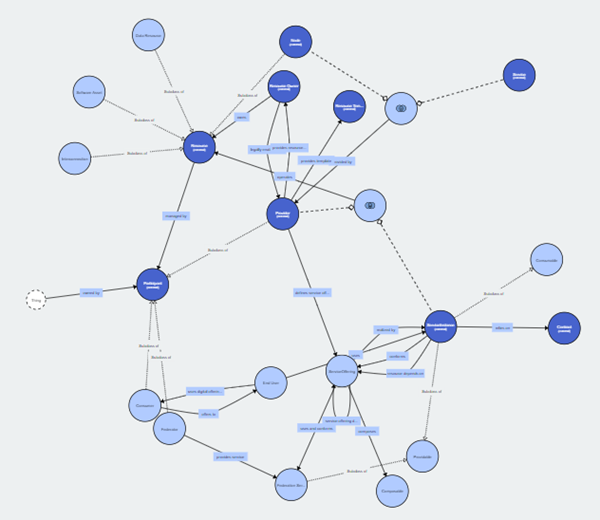
\includegraphics[width=0.7\linewidth]{introduction/figures/ontology_example.jpg}
   \end{center}
   \caption[Ontología: Ejemplo 1]
   {\footnotesize Ontología: Ejemplo 1}
   \label{fig:mufigure6}
\end{figure}

En la Figura 2, podemos ver una estructura de datos en la cual cada concepto está representado por un círculo, y entre ellos están conectados por diferentes tipos de líneas, para diferenciar las relaciones.

\begin{figure}[ht]
   \begin{center}
      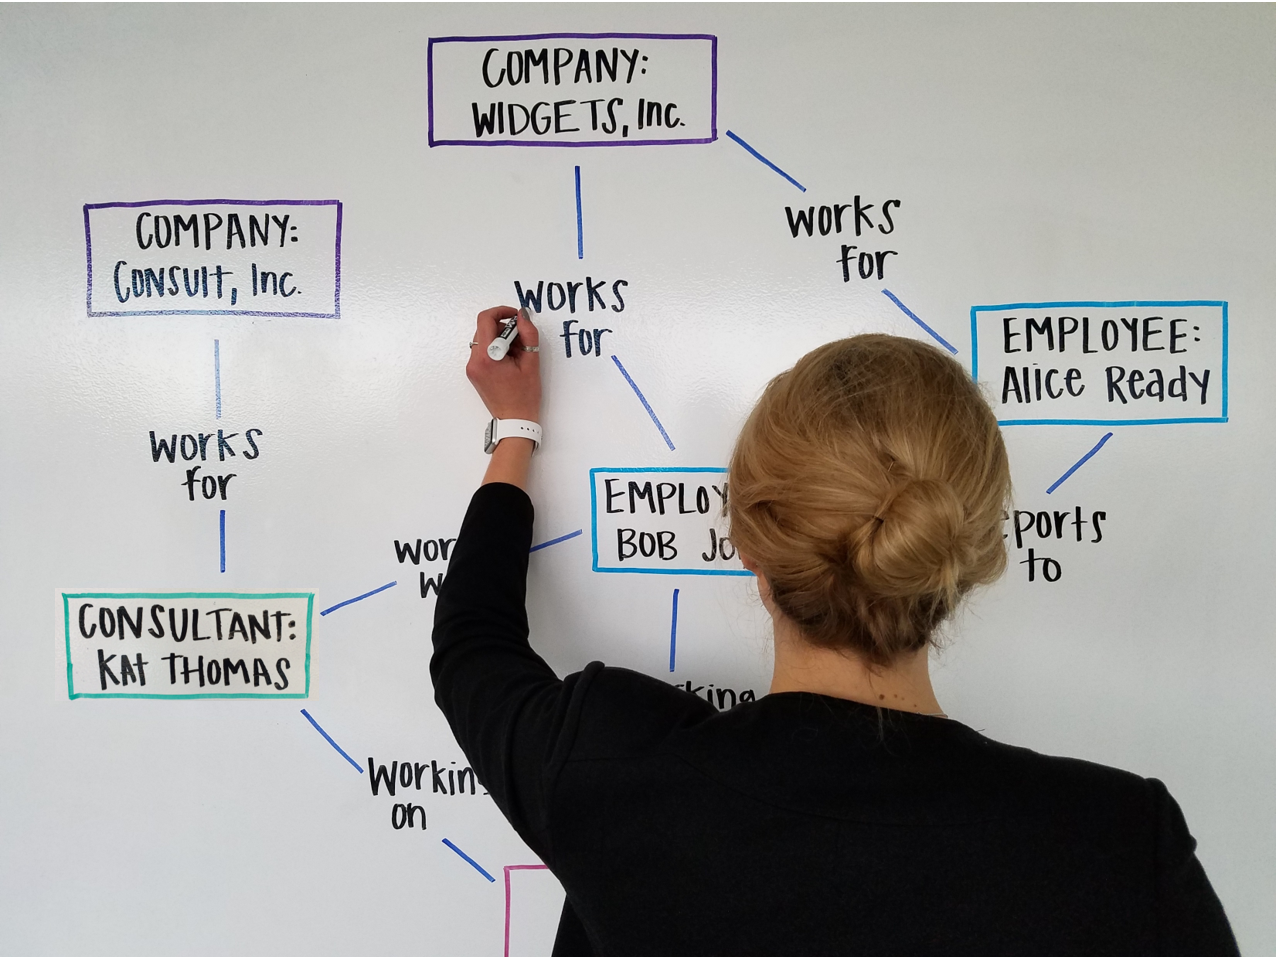
\includegraphics[width=0.7\linewidth]{introduction/figures/ontology_example_2.png}
   \end{center}
   \caption[Ontología: Ejemplo 2]
   {\footnotesize Ontología: Ejemplo 2}
   \label{fig:mufigure6}
\end{figure}

En la Figura 3, vemos como una empresa puede ser representada a través de ontologías al representar sus componentes como clases.

\begin{figure}[ht]
   \begin{center}
      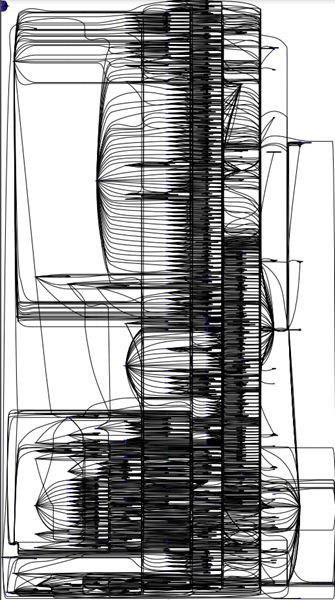
\includegraphics[width=0.4\linewidth]{introduction/figures/ontology_example_3.jpg}
   \end{center}
   \caption[Ontología: Ejemplo 3]
   {\footnotesize Ontología: Ejemplo 3}
   \label{fig:mufigure7}
\end{figure}

Para introducir de a poco la problématica que queremos enfrentar, podemos ver la Figura 4, que muestra qué tan compleja se puede ver una ontología si la cantidad de clases y relaciones incrementa demasiado.
Esta idea la iremos expandiendo un poco más en otras secciones.

\section{Gaia-X}

Gaia-X es una iniciativa que desarrolla, sobre la base de los valores europeos, una gobernanza digital que puede aplicarse a cualquier pila tecnológica existente de nube para obtener transparencia, controlabilidad, portabilidad e interoperabilidad entre datos y servicios. \cite[]{Gaiax}

\begin{figure}[ht]
   \begin{center}
      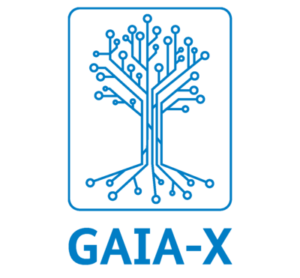
\includegraphics[width=0.4\linewidth]{introduction/figures/gaia-x.png}
   \end{center}
   \caption[Logo de Gaia-X]
   {\footnotesize Logo de Gaia-X}
   \label{fig:mufigure7}
\end{figure}

Hoy en día, muchos negocios de pequeña y mediana dimensión desarrollan interfaces individualmente para cada cliente para el intercambio de información y la interoperabilidad de soluciones. Esto cuesta tiempo y dinero. Gaia-X busca proveer mecanismos comunes de intercambio de información que adhieran a las necesidades comunes de confianza.

En Europa, la adopción de tecnologías de nube es solo del 26\%. Esto implica que la mayor parte de la información y de las aplicaciones son todavía inaccesibles e inintercambiables. Gaia-X desarrollará una estructura de trabajo que le permita a la gente tomar decisiones informadas a la hora de intercambiar información. 

¿Por qué están relacionados este proyecto y las ontologías? La descripción de entidades ha sido siempre uno de los objetivos de la informática. En primer lugar, porque ayuda a comprender la entidad descrita, y después porque su análisis sintáctico permite aplicar reglas y construir funcionalidades.

El objetivo de la ontología es ser abierta y compartida: describe lo que son las cosas en general, no en un contexto específico. De este modo se simplifica el proceso de diseño de nuevas ontologías, ya que se puede recurrir a las existentes, y también se facilita la interacción con otras organizaciones, porque se utilizan las mismas ontologías.

Por último, y quizá el punto más crucial, la ontología puede ser analizada fácilmente por una máquina, lo que facilita el razonamiento. \cite[]{GaiaxOntology}

El desarrollo del proyecto Gaia-X naturalmente va a depender de las ontologías y los softwares requeridos, por esta razón tenemos que asegurarnos de contar con herramientas adecuadas.
